% # 公立はこだて未来大学・修士論文テンプレートファイル(unicode)
%
% ## 改訂履歴:
% - 2019/12/01 初版 作成者:三上貞芳
% - 2020/12/16 修正版, funstyle_master.tex のエラー修正 作成者:髙橋佑太
% ## 論文作成の手順
%
% 1. 以下のtexファイルを作成してください
% - cover.tex           氏名・タイトル等の表紙情報
% - eabstract.tex       英語アブストラクト
% - jabstract.tex       日本語アブストラクト
% - chapterX.tex        本文第X章
% - publications.tex    発表・採録等の実績(確定分も含む)
% - acknowledgment.tex  謝辞
% - bibliography    .tex    参考文献
%
% 2. このテンプレートの「TODO: 本文」以下に,作成した章に対応する\input{chapterX.tex}文を追記してください(Xは章番号)
%
% 3. このテンプレートとfunstyle_master.texと合わせてuplatex環境でコンパイルし,PDFを作成します.
%

\documentclass[uplatex, a4paper, report, 11pt, oneside]{jsbook}

% packages
\usepackage[utf8]{inputenc}
\usepackage[dvipdfmx]{graphicx}
\usepackage{lmodern}             % use latin modern font
\usepackage{amsmath,amssymb,amsthm}

\usepackage{layout}

% 未来大書式設定
% # 公立はこだて未来大学・修士論文書式定義ファイル
%
% (https://github.com/kmiya/naist-thesis-tmpl を一部参照)
% 
% ## 改訂履歴:
% - 2019/11/18 初版 作成者:三上貞芳

% ## 使用法;
% - main.texを参照してください.
% - **このファイルを変更する必要はありません**

\usepackage[dvipdfmx]{graphicx}
\usepackage[utf8]{inputenc}
\usepackage[T1]{fontenc}
\usepackage{lmodern}
\usepackage{amsmath,amssymb,amsthm}
\usepackage{layout}
\let\equation\gather
\let\endequation\endgather
\usepackage{fancybox}
\usepackage[flushmargin,symbol]{footmisc}
\usepackage[nottoc]{tocbibind}
\usepackage[dvipdfmx,%
 bookmarks=true,%
 bookmarksnumbered=true,%
 setpagesize=false,%
 colorlinks=false,%
 linkbordercolor={0.8 0.8 0.8},%
 citebordercolor={0.8 0.8 0.8},%
 pdfborder={0 0 0.6},%
% urlcolor=black,linkcolor=black,citecolor=black,%
 pdftitle={\etitle},
 pdfauthor={\eauthor},
 pdfsubject={\edoctitle},
 pdfkeywords={\ekeywords}
]{hyperref}
\usepackage{pxjahyper}

% ページレイアウト
\textheight=20.6truecm          % 縦
\textwidth=14.5truecm           % 横
\oddsidemargin=0.6truecm        % 左マージン(1inオフセット後)
\evensidemargin=-3.8truecm      % 右マージン(1inオフセット後)

% フォント等調整
% 参考文献
\def\thebibliography#1{
  \chapter*{
    参考文献\markboth{参 考 文 献}{参 考 文 献}
    % \addcontentsline{toc}{chapter}{参考文献} % エラーのため,\addcontentsline は main.tex に移動.
  }
  \list{[\arabic{enumi}]}{\settowidth\labelwidth{[#1]}\leftmargin\labelwidth
  \advance\leftmargin\labelsep
  \usecounter{enumi}}
  % \def\newblock{\hskip .11trueem plus .33trueem minus -.07trueem} % エラーのため削除
  \sloppy
  \sfcode`\.=1000\relax
}
\let\endthebibliography=\endlist

% 章
\makeatletter%%
\def\@makechapterhead#1{\hbox{}%
  \vskip-1\Cvs
  {\parindent\z@
%  \reset@font\LARGE\bfseries
   \raggedright\reset@font\Large\bfseries% 左揃え
   \ifnum \c@secnumdepth >\m@ne
     \setlength\@tempdima{\linewidth}%
     \vtop{\hsize\@tempdima%
         \@chapapp\thechapter\@chappos\mbox{\ \ }%
     #1}%
   \else
     #1\relax
   \fi}\nobreak\vskip1\Cvs}
\makeatother%%

\makeatletter%%
\def\@makeschapterhead#1{\hbox{}%
  \vskip-1\Cvs
  {\parindent \z@ \raggedright
    \normalfont
    \interlinepenalty\@M
    \Large\headfont #1\par\nobreak
    \vskip1\Cvs}}
\makeatother%%

% 節
\makeatletter%%
\renewcommand{\section}{%
  \@startsection{section}% #1 見出し
   {1}% #2 見出しのレベル
   {\z@}% #3 横組みの場合,見出し左の空き(インデント量)
   {1.5\Cvs \@plus.5\Cdp \@minus.2\Cdp}% #4 見出し上の空き
   {.5\Cvs \@plus.3\Cdp}% #5 見出し下の空き (負の値なら見出し後の空き)
  {\raggedright\reset@font\large\bfseries}% 左揃え
}%
\makeatother%%

% 小節
\makeatletter%%
\renewcommand{\subsection}{%
  \@startsection{subsection}% #1 見出し
   {1}% #2 見出しのレベル
   {\z@}% #3 横組みの場合,見出し左の空き(インデント量)
   {1.5\Cvs \@plus.5\Cdp \@minus.2\Cdp}% #4 見出し上の空き
   {.5\Cvs \@plus.3\Cdp}% #5 見出し下の空き (負の値なら見出し後の空き)
  {\raggedright\reset@font\normalsize\bfseries}% 左揃え
}%
\makeatother%%

% 表題
\makeatletter
\def\@startsection#1#2#3#4#5#6{%
  \if@noskipsec \leavevmode \fi
  \par
  \@tempskipa #4\relax
  \if@english \@afterindentfalse \else \@afterindenttrue \fi
  \ifdim \@tempskipa <\z@
    \@tempskipa -\@tempskipa \@afterindentfalse
  \fi
  \if@nobreak
    \everypar{}%
  \else
    \addpenalty\@secpenalty
    \ifdim \@tempskipa >\z@
      \vskip\@tempskipa
      \if@slide\else
        \null
        \vspace{-\baselineskip}%
      \fi
    \fi
  \fi
  \noindent
  \@ifstar
    {\@ssect{#3}{#4}{#5}{#6}}%
    {\@dblarg{\@sect{#1}{#2}{#3}{#4}{#5}{#6}}}}
\makeatother

% 式番号
\makeatletter
  \renewcommand{\theequation}{%
  \thesection.\arabic{equation}}
    \@addtoreset{equation}{section}
\makeatother


% 図番号
\makeatletter
 \renewcommand{\thefigure}{%
  \thechapter.\arabic{figure}}
   \@addtoreset{figure}{chapter}
 \makeatother
\makeatletter

% 目次に小節を表示
\setcounter{tocdepth}{4}


% TODO: タイトル・著者等の情報
% TODO: 論文題目等の情報を以下に記入

\newcommand{\jdoctitle}{修士論文}
\newcommand{\edoctitle}{Master's Thesis}
\newcommand{\jtitle}{未来大修士論文日本語題目サンプル}  % 修論の題名
\newcommand{\etitle}{Lorem Ipsum Dolor sit Amet Consectetuer Adipiscing Elit}   % 論文題目(英)
\newcommand{\jauthor}{姓 名}      % 著者名(日)
\newcommand{\eauthor}{Firstname Lastname} % 著者名(英)
\newcommand{\jadvisor}{姓 名}   % 指導教員名(日)
\newcommand{\eadvisor}{Firstname Lastname}  % 指導教員名(英)
\newcommand{\jdate}{20XX年2月XX日}  % 論文提出日   (日)
\newcommand{\edate}{February XX, 20XX}  % 論文提出年月 (英)
\newcommand{\jkeywords}{キーワード1, キーワード2, キーワード3} % キーワード(日)
\newcommand{\ekeywords}{Keyword1, Keyword2, Keyword3}   % キーワード(英)
\newcommand{\eshorttitle}{Your Short English Title Here}    % 短縮英題題名(おおよそ8 words以内)
\newcommand{\jaffiliation}{知能情報科学領域}    % 領域名(日)
\newcommand{\eaffiliation}{Intelligent Information Science Area}    % 領域名(英)


% TODO: 英語アブストラクト
% TODO: 英文アブストラクトを以下の{}内に記述(以下はダミーテキスト)
\newcommand{\eabstract}{

(Abstract must be within 1 page. Following is a sample text.)
Lorem ipsum dolor sit amet, consectetuer adipiscing elit. Maecenas porttitor congue massa. Fusce posuere, magna sed pulvinar ultricies, purus lectus malesuada libero, sit amet commodo magna eros quis urna.
Nunc viverra imperdiet enim. Fusce est. Vivamus a tellus.
Pellentesque habitant morbi tristique senectus et netus et malesuada fames ac turpis egestas. Proin pharetra nonummy pede. Mauris et orci.
Aenean nec lorem. In porttitor. Donec laoreet nonummy augue.
Suspendisse dui purus, scelerisque at, vulputate vitae, pretium mattis, nunc. Mauris eget neque at sem venenatis eleifend. Ut nonummy.
Lorem ipsum dolor sit amet, consectetuer adipiscing elit. Maecenas porttitor congue massa. Fusce posuere, magna sed pulvinar ultricies, purus lectus malesuada libero, sit amet commodo magna eros quis urna.
Nunc viverra imperdiet enim. Fusce est. Vivamus a tellus.
Pellentesque habitant morbi tristique senectus et netus et malesuada fames ac turpis egestas. Proin pharetra nonummy pede. Mauris et orci.
Aenean nec lorem. In porttitor. Donec laoreet nonummy augue.
Suspendisse dui purus, scelerisque at, vulputate vitae, pretium mattis, nunc. Mauris eget neque at sem venenatis eleifend. Ut nonummy.

}

% TODO: 日本語アブストラクト
% TODO: 日本語アブストラクトを以下の{}内に記述(以下はダミーテキスト)
\newcommand{\jabstract}{

(1ページ以内に収めること.以下はダミーテキスト)
ビデオを使うと,伝えたい内容を明確に表現できます.[オンライン ビデオ] をクリックすると,追加したいビデオを,それに応じた埋め込みコードの形式で貼り付けできるようになります.キーワードを入力して,文書に最適なビデオをオンラインで検索することもできます.
Word に用意されているヘッダー,フッター,表紙,テキスト ボックス デザインを組み合わせると,プロのようなできばえの文書を作成できます.たとえば,一致する表紙,ヘッダー,サイドバーを追加できます.[挿入] をクリックしてから,それぞれのギャラリーで目的の要素を選んでください.
テーマとスタイルを使って,文書全体の統一感を出すこともできます.[デザイン] をクリックし新しいテーマを選ぶと,図やグラフ,SmartArt グラフィックが新しいテーマに合わせて変わります.スタイルを適用すると,新しいテーマに適合するように見出しが変更されます.
Word では,必要に応じてその場に新しいボタンが表示されるため,効率よく操作を進めることができます.文書内に写真をレイアウトする方法を変更するには,写真をクリックすると,隣にレイアウト オプションのボタンが表示されます.表で作業している場合は,行または列を追加する場所をクリックして,プラス記号をクリックします.

}

% page size
\textheight     = 22.6truecm
\textwidth      = 14.7truecm
\oddsidemargin  = 0.6truecm

% header and footer
\usepackage{fancyhdr}
\pagestyle{fancy}
\setlength{\footskip}{16pt}
\fancyhf{}
\renewcommand{\chaptermark}[1]{\markboth{\thechapter.\ #1}{}}
\rhead{\leftmark}
\renewcommand{\headrulewidth}{0pt}
\cfoot{\thepage}
\lfoot{~~ \\Master's thesis, Future University Hakodate}
\lhead{\eshorttitle}

%-------------------------------------
\begin{document}
\thispagestyle{empty}
\vspace*{1.5truemm}
\begin{center}
    \LARGE\bfseries
    修士論文
\end{center}
\vspace*{2truemm}
\begin{center}
    \LARGE\bfseries\jtitle
\end{center}
\vspace*{2em}
\begin{center}
    \large\bfseries 公立はこだて未来大学大学院~~システム情報科学研究科\par%
    \jaffiliation
\end{center}
\vspace*{1em}
\begin{center}
    \Large\bfseries\jauthor
\end{center}
\vspace*{1em}
\begin{center}
    \large 指導教員~~~~\jadvisor\par
    \vspace{0.5em}
    \large 提出日~~~~\jdate
\end{center}
\vspace*{3em}
\begin{center}
\textbf{\Large Master's Thesis}\par
\vspace*{2em}
\textbf{\Large \etitle}\par
\vspace*{1em}
{\normalsize by}\par
\vspace*{1em}
{\large \eauthor}\par
\vspace*{1.5em}
Graduate School of Systems Information Science, Future University Hakodate \par
\eaffiliation

% \vspace*{0.5em}
\normalsize Supervisor: \quad \eadvisor \par
\vspace*{2em}
Submitted on \edate
\end{center}
%\vspace*{\fill}

% 英語アブストラクト作成
\newpage
\thispagestyle{empty}
\vspace*{30truemm}
\noindent
\textbf{Abstract--}~
\eabstract

\vspace*{1em}
\noindent
\textbf{Keywords:}~ 
\ekeywords

% 日本語アブストラクト作成
\newpage
\thispagestyle{empty}
\vspace*{30truemm}
\noindent
\textgt{概~要:}~
\jabstract

\vspace*{1em}
\noindent
\textgt{キーワード:}~ 
\jkeywords

% 目次
\tableofcontents
\thispagestyle{empty}

% ページ番号初期化
\setcounter{page}{0}

% TODO: 本文
% input chapters
\chapter{序論}	% TODO: 章題を記入.題は任意.
\thispagestyle{plain}   % chapterの直後に必ず指定

% input sections
\section{はじめに}
ビデオを使うと,伝えたい内容を明確に表現できます.[オンライン ビデオ] をクリックすると,追加したいビデオを,それに応じた埋め込みコードの形式で貼り付けできるようになります.キーワードを入力して,文書に最適なビデオをオンラインで検索することもできます.
\section{目的}
ビデオを使うと,伝えたい内容を明確に表現できます.[オンライン ビデオ] をクリックすると,追加したいビデオを,それに応じた埋め込みコードの形式で貼り付けできるようになります.キーワードを入力して,文書に最適なビデオをオンラインで検索することもできます.
\section{章構成}

ビデオを使うと,伝えたい内容を明確に表現できます.[オンライン ビデオ] をクリックすると,追加したいビデオを,それに応じた埋め込みコードの形式で貼り付けできるようになります.キーワードを入力して,文書に最適なビデオをオンラインで検索することもできます.

Word に用意されているヘッダー,フッター,表紙,テキスト ボックス デザインを組み合わせると,プロのようなできばえの文書を作成できます.たとえば,一致する表紙,ヘッダー,サイドバーを追加できます.[挿入] をクリックしてから,それぞれのギャラリーで目的の要素を選んでください.
テーマとスタイルを使って,文書全体の統一感を出すこともできます.[デザイン] をクリックし新しいテーマを選ぶと,図やグラフ,SmartArt グラフィックが新しいテーマに合わせて変わります.スタイルを適用すると,新しいテーマに適合するように見出しが変更されます.

Word では,必要に応じてその場に新しいボタンが表示されるため,効率よく操作を進めることができます.文書内に写真をレイアウトする方法を変更するには,写真をクリックすると,隣にレイアウト オプションのボタンが表示されます.表で作業している場合は,行または列を追加する場所をクリックして,プラス記号をクリックします.

新しい閲覧ビューが導入され,閲覧もさらに便利になりました.文書の一部を折りたたんで,必要な箇所に集中することができます.最後まで読み終わる前に中止する必要がある場合,Word では,たとえ別のデバイスであっても,どこまで読んだかが記憶されます.

\begin{figure}
    \centering
    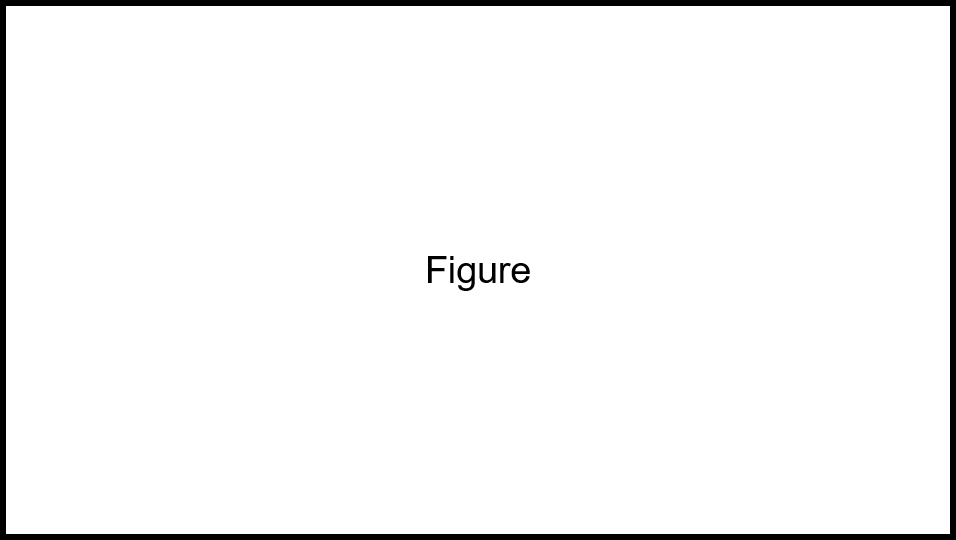
\includegraphics[width=0.7\textwidth]{fig1.png}
    \caption{図のキャプション}
    \label{fig:my_label}
\end{figure}

ビデオを使うと,伝えたい内容を明確に表現できます.[オンライン ビデオ] をクリックすると,追加したいビデオを,それに応じた埋め込みコードの形式で貼り付けできるようになります.キーワードを入力して,文書に最適なビデオをオンラインで検索することもできます.

Word に用意されているヘッダー,フッター,表紙,テキスト ボックス デザインを組み合わせると,プロのようなできばえの文書を作成できます.たとえば,一致する表紙,ヘッダー,サイドバーを追加できます.[挿入] をクリックしてから,それぞれのギャラリーで目的の要素を選んでください.
テーマとスタイルを使って,文書全体の統一感を出すこともできます.[デザイン] をクリックし新しいテーマを選ぶと,図やグラフ,SmartArt グラフィックが新しいテーマに合わせて変わります.スタイルを適用すると,新しいテーマに適合するように見出しが変更されます.

Word では,必要に応じてその場に新しいボタンが表示されるため,効率よく操作を進めることができます.文書内に写真をレイアウトする方法を変更するには,写真をクリックすると,隣にレイアウト オプションのボタンが表示されます.表で作業している場合は,行または列を追加する場所をクリックして,プラス記号をクリックします.

新しい閲覧ビューが導入され,閲覧もさらに便利になりました.文書の一部を折りたたんで,必要な箇所に集中することができます.最後まで読み終わる前に中止する必要がある場合,Word では,たとえ別のデバイスであっても,どこまで読んだかが記憶されます.

\begin{table}[htb]
    \caption{表のキャプション}
    \centering
    \begin{tabular}{lcr}
        \hline
        head1 & head2 & head3 \\
        \hline\hline
        123 & 456 & 789\\
        \hline
    \end{tabular}
    \label{tab:my_label}
\end{table}

ビデオを使うと,伝えたい内容を明確に表現できます.[オンライン ビデオ] をクリックすると,追加したいビデオを,それに応じた埋め込みコードの形式で貼り付けできるようになります.キーワードを入力して,文書に最適なビデオをオンラインで検索することもできます.

Word に用意されているヘッダー,フッター,表紙,テキスト ボックス デザインを組み合わせると,プロのようなできばえの文書を作成できます.たとえば,一致する表紙,ヘッダー,サイドバーを追加できます.[挿入] をクリックしてから,それぞれのギャラリーで目的の要素を選んでください.
テーマとスタイルを使って,文書全体の統一感を出すこともできます.[デザイン] をクリックし新しいテーマを選ぶと,図やグラフ,SmartArt グラフィックが新しいテーマに合わせて変わります.スタイルを適用すると,新しいテーマに適合するように見出しが変更されます.

Word では,必要に応じてその場に新しいボタンが表示されるため,効率よく操作を進めることができます.文書内に写真をレイアウトする方法を変更するには,写真をクリックすると,隣にレイアウト オプションのボタンが表示されます.表で作業している場合は,行または列を追加する場所をクリックして,プラス記号をクリックします.
新しい閲覧ビューが導入され,閲覧もさらに便利になりました.文書の一部を折りたたんで,必要な箇所に集中することができます.最後まで読み終わる前に中止する必要がある場合,Word では,たとえ別のデバイスであっても,どこまで読んだかが記憶されます.

ビデオを使うと,伝えたい内容を明確に表現できます.[オンライン ビデオ] をクリックすると,追加したいビデオを,それに応じた埋め込みコードの形式で貼り付けできるようになります.キーワードを入力して,文書に最適なビデオをオンラインで検索することもできます.

Word に用意されているヘッダー,フッター,表紙,テキスト ボックス デザインを組み合わせると,プロのようなできばえの文書を作成できます.たとえば,一致する表紙,ヘッダー,サイドバーを追加できます.[挿入] をクリックしてから,それぞれのギャラリーで目的の要素を選んでください.
テーマとスタイルを使って,文書全体の統一感を出すこともできます.[デザイン] をクリックし新しいテーマを選ぶと,図やグラフ,SmartArt グラフィックが新しいテーマに合わせて変わります.スタイルを適用すると,新しいテーマに適合するように見出しが変更されます.

Word では,必要に応じてその場に新しいボタンが表示されるため,効率よく操作を進めることができます.文書内に写真をレイアウトする方法を変更するには,写真をクリックすると,隣にレイアウト オプションのボタンが表示されます.表で作業している場合は,行または列を追加する場所をクリックして,プラス記号をクリックします.

新しい閲覧ビューが導入され,閲覧もさらに便利になりました.文書の一部を折りたたんで,必要な箇所に集中することができます.最後まで読み終わる前に中止する必要がある場合,Word では,たとえ別のデバイスであっても,どこまで読んだかが記憶されます.



% TODO: 謝辞
\chapter*{謝辞}
\thispagestyle{plain}
% \addcontentsline{toc}{chapter}{謝辞} % 目次に入れたい場合は有効にする

% TODO: 謝辞を以下に記入
関係各位様に感謝いたします.


% TODO: 発表等実績
\chapter*{発表・採録実績}
\thispagestyle{plain}
\addcontentsline{toc}{chapter}{発表・採録実績} % 目次に入れたい場合は有効にする

% TODO: 発表・採録実績(確定分も含む)を以下の例のように記入

\subsection*{発表等}
\begin{enumerate}
\renewcommand{\labelenumi}{[\arabic{enumi}]}
    \item 発表その1
    \item 発表その2
    \item 発表予定(発表予定年月)
\end{enumerate}

\subsection*{学術論文,国際会議等(査読付き)}
\begin{enumerate}
\renewcommand{\labelenumi}{[\arabic{enumi}]}
    \item 論文その1
    \item 国際会議その1
    \item 採録決定論文(採録予定年月)
\end{enumerate}

% TODO: 参考文献
% % TODO: 参考文献を以下のように記入.

\begin{thebibliography}{99}
 \bibitem{item1}
Reference1
 \bibitem{item2}
Reference2
\end{thebibliography}
 % 手書きでbibliographyを入力する場合
\bibliographystyle{acm} % bibTeXから自動生成する場合 styles: https://www.overleaf.com/learn/latex/Bibtex_bibliography_styles
\bibliography{references} % bibTeXから自動生成する場合
\thispagestyle{plain}
\addcontentsline{toc}{chapter}{参考文献} % 目次に参考文献を出力する(funstyle_master.texから移動)

bibTeXを使う場合は最低1つciteしないとエラーが発生するので注意.\cite{kuzmanovic2003low} % TODO: remove this line.

% 図表一覧等自動生成
\listoffigures
\thispagestyle{plain}
\listoftables
\thispagestyle{plain}


\end{document}
